\setchapterpreamble[u]{\margintoc}
\chapter{\textit{ColPali}: Efficient Document Retrieval with Vision Language Models}

% \begin{figure*}[ht] 
%     \centering
% ¡    \includegraphics[width = 0.95\textwidth]{images/colpali_images/architecture.png}
%     \caption{}
%     \label{fig:colpali_architecture}
% \end{figure*}
\begin{kaobox}[frametitle=Paper Abstract]


Documents are visually rich structures that convey information through text, but also figures, page layouts, tables, or even fonts. Since modern retrieval systems mainly rely on the textual information they extract from document pages to index documents -often through lengthy and brittle processes-, they struggle to exploit key visual cues efficiently. This limits their capabilities in many practical document retrieval applications such as Retrieval Augmented Generation (RAG).
To benchmark current systems on visually rich document retrieval, we introduce the Visual Document Retrieval Benchmark \textit{ViDoRe}, composed of various page-level retrieval tasks spanning multiple domains, languages, and practical settings. 
The inherent complexity and performance shortcomings of modern systems motivate a new concept; doing document retrieval by directly embedding the images of the document pages. We release \textit{ColPali}, a Vision Language Model trained to produce high-quality multi-vector embeddings from images of document pages. Combined with a late interaction matching mechanism, \textit{ColPali} largely outperforms modern document retrieval pipelines while being drastically simpler, faster and end-to-end trainable. 
We release models, data, code and benchmarks under open licenses at \url{https://hf.co/vidore}.


\end{kaobox}


\section{Introduction}

Document Retrieval consists of matching a user query to relevant documents in a given corpus. It is central to many widespread industrial applications, either as a standalone ranking system (search engines) or as part of more complex information extraction or Retrieval Augmented Generation (RAG) pipelines.

%\vspace{0.1cm}
% Historically, statistical methods based on word frequencies were used (e.g. TF-IDF \sidecite{sparck_jones_idf_2004}, BM25 \sidecite{robertson_probabilistic_2009}), enabling offline corpus indexation in sparse vector sets, and fast query matching at inference time. With the advent of neural networks, stronger dense embedding models were developed by fine-tuning pre-trained language models with contrastive training objectives \sidecite{cer_universal_2018,reimers_sentence-bert_2019,gao_simcse_2021}. 


% Although text embedding models for query-passage retrieval have greatly improved over recent years, notably enabled by the rise of pretrained language models, the main bottleneck for efficient document retrieval in a practical industrial setting lies \textit{a priori}, in the way text passages to be embedded are constructed.

\noindent Over recent years, pretrained language models have enabled large improvements in text embedding models. In practical industrial settings, however, the primary performance bottleneck for efficient document retrieval stems not from embedding model performance but from the prior data ingestion pipeline. Indexing a standard PDF document involves several steps. First, PDF parsers or Optical Character Recognition (OCR) systems are used to extract words from the pages. Document layout detection models can then be run to segment paragraphs, titles, and other page objects such as tables, figures, and headers. A chunking strategy is then defined to group text passages with some semantical coherence, and modern retrieval setups may even integrate a captioning step to describe visually rich elements in a natural language form, more suitable for embedding models. 
% This leads to ingestion pipelines that are lengthy, require heavy parametrization, and orchestrate independent subsystems. 
In our experiments (\autoref{table:colpali:results}), we typically find that optimizing the ingestion pipeline yields much better performance on visually rich document retrieval than optimizing the text embedding model.


% The race to ever-more performant text embedding models should perhaps not be the only focus of research in the retrieval space.

% pipeline usually starts with a rotation correction model. Then comes the Optical Character Recognition (OCR) task: a text detection model locates the character/word bounding boxes (e.g. \texttt{crnn\_vgg16\_bn} \sidecite{shi_end--end_2015}, \texttt{LinkNet} \sidecite{chaurasia_linknet_2017}, \texttt{TextNET \sidecite{chen_fast_2021}}) and a text recognition model predicts the strings associated the words in the previously detected bounding boxes (e.g. \texttt{db\_resnet50}, \texttt{db\_mobilenet\_v3\_large} \sidecite{liao_real-time_2019}, \texttt{sar\_resnet31} \sidecite{li_show_2018}). Finally, specialized models or heuristics to determine the reading order to segment pages into titles and paragraphs \sidecite{huang_layoutlmv3_2022,meunier_optimized_2005}, to detect images and tables \sidecite{smock_pubtables-1m_2021,qiao_lgpma_2021,li_dit_2022,ge_yolox_2021} in order to process them separately, and finally to split documents into optimized text chunks to be embedded. The whole process can be lengthy, and its sequential nature propagates errors from earlier systems downstream. Moreover, it is non-differentiable and requires heavy parametrization efforts to optimize the deployment infrastructures. Finally, it is unclear how to best represent visually rich document objects such as tables, figures, and images \sidecite{zha_tablegpt_2023,gao_retrieval-augmented_2023}. In practice, they are often overlooked, although recently, some captioning strategies have been shown to be effective, although very resource-intensive during indexation.

\noindent\textbf{Contribution 1: \textit{ViDoRe}.}
In this work, we argue that document retrieval systems should not be evaluated solely on the capabilities of text embedding models \sidecite{bajaj_ms_2016,thakur_beir_2021, muennighoff_mteb_2022}, but should also consider the context and visual elements of the documents to be retrieved. To this end, we create and openly release \textit{ViDoRe}, a comprehensive benchmark to evaluate systems on page-level document retrieval with a wide coverage of domains, visual elements, and languages. \textit{ViDoRe} addresses practical document retrieval scenarios, where queries often necessitate both textual and visual understanding for accurate document matching. We highlight the shortcomings of current text-centric systems in these settings.\sidenote{The \textit{ViDoRe} benchmark leaderboard is hosted publicly at \url{https://huggingface.co/spaces/vidore/vidore-leaderboard} to encourage further developments.}

% \url{https://huggingface.co/spaces/<anonymous>}

\noindent\textbf{Contribution 2: \textit{ColPali}.}
We propose a novel concept and model architecture based on Vision Language Models (VLMs) to efficiently index documents purely from their visual features, allowing for subsequent fast query matching with late interaction mechanisms \sidecite{khattab_colbert_2020}. Our method, \textit{ColPali}, significantly outperforms all other retrieval systems on \textit{ViDoRe} while being fast and end-to-end trainable.
These results demonstrate the potential and the many benefits of this novel \textit{Retrieval in Vision Space} concept, which could significantly alter the way document retrieval is approached in the industry moving forward.
We release all resources at \url{https://hf.co/vidore}.

% \url{https://hf.co/<anonymous>}

% We argue this has the potential to revolutionize
% \sidenote{All project artifacts are openly released at \url{.com}.}.

% pour moi overclaim. New method =`> des insights. Ca fait croqueur
% \textbf{Contribution 3.}
% We run ablations to better understand the impact of our modeling choices on the retrieval performances. This unlocks insights into the trade-offs between model size and the number of image patches, as well as informs on the impact of design decisions, such as locked-image tuning, memory tokens, loss functions, etc...

% \textbf{Contribution 4.}
% We release our fine-tuned models and training code under open licenses, bringing to both researchers and industry practitioners state-of-the-art document retrieval models\sidenote{\url{huggingface.co/anon}}. We also release all artifacts related to benchmarking\sidenote{\url{github.com/anon}} (data, evaluation code, public leaderboards, reproducible baselines) to serve as a new reference for Document Retrieval.

\begin{figure*}
    \centering
    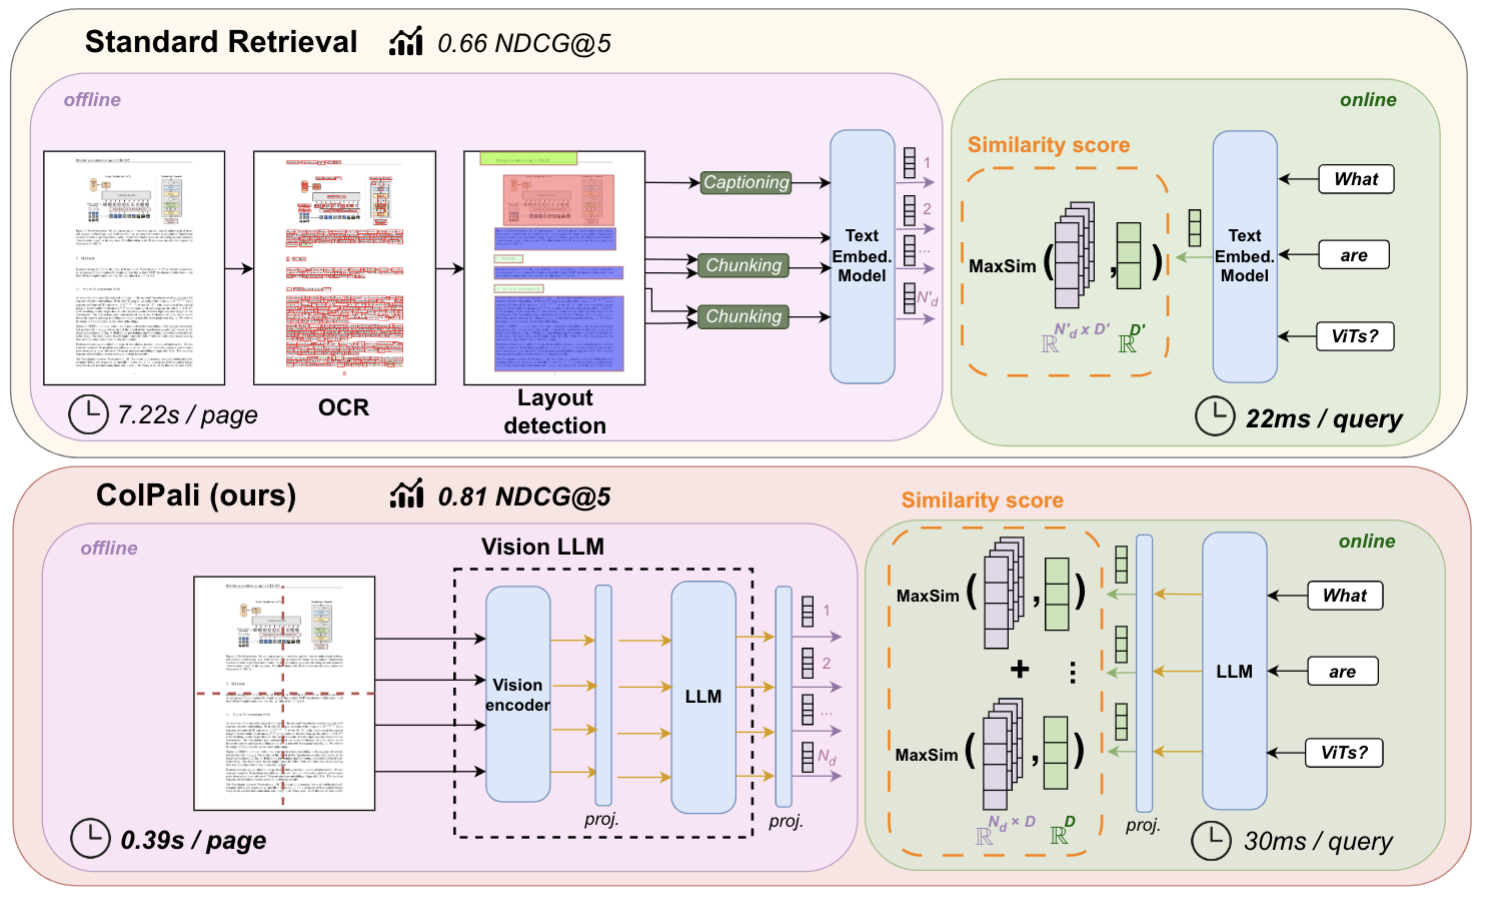
\includegraphics[width = 1.2\textwidth]{images/colpali_images/final_architecture.png}
    \caption[\textit{ColPali} overview]{\textit{ColPali} simplifies document retrieval w.r.t. standard retrieval methods while achieving stronger performances with better latencies. Latencies and results are detailed in \autoref{section:colpali:results} and \autoref{paragraph:latency_app}.}
    
    % Latencies indicated in the figure are computed on the same machine \texttt{g2-standard-16} with a NVIDIA-L4 GPU, and averaged over 100 pages. Further details in \autoref{subsection:latency}.The computed score is the average of from all datasets in \textit{ViDoRe} for PDF Parser + Captioning and ColPali respectively. Further details in \autoref{section:results}.} 
    \label{fig:colpali_architecture}
\end{figure*}


\section{Problem Formulation \& Related Work}

% Pierre
\noindent\textbf{Problem Setting.}
In our setting, a retrieval system scores how relevant a document $d$ from corpus $\mathcal{D}$ is with respect to a query $q$. Computing the similarity score $s(q, d) \in \mathbb{R}$ for each of the $|\mathcal{D}|$ documents in the corpus creates a ranking we can use to extract the most relevant documents. In this work, we focus on page-level retrieval: \textit{given a query, is the correct document page retrieved by the system?} For coherence with existing literature, we further use the term \textit{document} to refer to individual pages, i.e.\ the atomic retrieved elements in our setting. As we focus on practical industrial retrieval applications (RAG, search engines) with potentially large corpora sizes, latency constraints are imposed on scoring systems. Most current retrieval systems can be decomposed into (1) an \textit{offline} indexation phase in which a document index is built and (2) an \textit{online} querying phase in which a query is matched to documents from the index and where low latency is vital to the user experience. 

% \noindent\textbf{Efficient document retrieval systems exhibit joint properties of high retrieval performance (R1), low latency during querying (R2), and high throughput during indexation (R3).}

\label{subsec:constraints}
\noindent\textit{Under these industrial constraints, we identify three main properties an efficient document retrieval systems should exhibit: \textbf{(R1) strong retrieval performance}, as measured by standard retrieval metrics; \textbf{(R2) fast online querying}, measured through average latencies; \textbf{(R3) high throughput corpus indexation}, ie. the number of pages that can be embedded in a given timeframe.}


\subsection{Textual Retrieval Methods}
\noindent\textbf{Document Retrieval in Text Space.}

Statistical methods based on word frequency like TF-IDF \sidecite{sparck_jones_statistical_1972} and BM25 \sidecite{robertson_okapi_1994} are still widely used due to their simplicity and efficiency. More recently, neural embedding models based on fine-tuned large language models display state-of-the-art performance on a variety of text embedding tasks and top the retrieval leaderboards \sidecite{muennighoff_mteb_2022}. 

\noindent\textbf{Neural Retrievers.}
In bi-encoder models \sidecite{reimers_sentence-bert_2019, karpukhin_dense_2020, wang_text_2022}, documents are independently mapped \textit{offline} to a dense vector space. Queries are embedded \textit{online} and matched to documents through a fast cosine distance computation.
A slower, but slightly more performant alternative, cross-encoder systems \sidecite{wang_minilm_2020, cohere_introducing_2024} concatenate query and document as a single input sequence and iteratively attribute matching scores to each possible combination. This enables full attention computation between query and document terms but comes at the cost of computational efficiency, as $|\mathcal{D}|$ encoding passes must be done online.


\noindent\textbf{Multi-Vector retrieval via late interaction.}
In the late interaction paradigm introduced by ColBERT \sidecite{khattab_colbert_2020}, an embedding is pre-computed and indexed per document token. At runtime, similarity can be computed with individual query token embeddings. The idea is to benefit from the rich interaction between individual query and document terms while taking advantage of the offline computation and fast query matching enabled by bi-encoders. See \autoref{subsection:glossary_colbert} for more details.

% introduces the late interaction paradigm, which consists of handling independent multi-vector representations of the query and the document. This method offers ColBERT two advantages. First, being able to compute the representation of the documents prior to the query (\textit{late interaction}) makes it suitable for offline document indexing, thus reducing latency at query time. On the other hand, the decision of having a document represented by not one but a sequence of vectors allows to fully leverage the expressiveness of the neural text encoder.

% Although benchmarks and leaderboards have been developed to evaluate these text embedding models (MTEB, BEIR), most of the performance improvements in practical use cases of embedding models depend on the prior data ingestion pipeline (OCR, layout detection, chunking strategies) and we believe end-to-end evaluation is crucial to accurately close the gap between academic model benchmarks and industrial performance.

\noindent\textbf{Retrieval Evaluation.}
Although benchmarks and leaderboards have been developed to evaluate text embedding models \sidecite{thakur_beir_2021, muennighoff_mteb_2022}, much of the performance improvements in industrial use cases of embedding models stem from the prior data ingestion pipeline. While documents often rely on visual elements to more efficiently convey information to human readers, text-only systems barely tap into these visual cues. Other work has also independently studied table or chart retrieval systems through repurposed Question Answering datasets \sidecite{Zhang_2019, nowak-etal-2024-multimodal} but only assessing specialized methods for each task.

\noindent\textit{To our knowledge, no benchmark evaluates document retrieval systems in practical settings; in an end-to-end manner, across several document types and topics, and by evaluating the use of both textual and visual document features.}



\subsection{Integrating Visual features}

\noindent\textbf{Contrastive Vision Language Models.}
Mapping latent representations of textual content to corresponding representations of visual content has been done by aligning disjoint visual and text encoders through contrastive losses \sidecite{radford_learning_2021, zhai_sigmoid_2023}. While some OCR capabilities exist in these models, the visual component is often not optimized for text understanding. 

The Fine-grained Interactive Language-Image Pre-training \sidecite{yao_filip_2021} framework extends the late interaction mechanism to cross-modal Vision Language Models, relying on max similarity operations between text tokens and image patches.


\noindent\textbf{Visually Rich Document Understanding.}
% While the document signal can be found in tables, images, and figures, it is also found in the document layout or even font sizes and colors. 
To go beyond text, some document-focused models jointly encode text tokens alongside visual or document layout features \sidecite{appalaraju_docformer_2021, kim_ocr-free_2021, huang_layoutlmv3_2022, tang_unifying_2022}. 
Large Language transformer Models (LLMs) with strong reasoning capabilities have recently been combined with Vision Transformers (ViTs) \sidecite{dosovitskiy_image_2020} to create VLMs \sidecite{alayrac_flamingo_2022, liu_visual_2023, bai_qwen-vl_2023, laurencon_what_2024} where image patch vectors from contrastively trained ViT models \sidecite{zhai_sigmoid_2023} are fed as input embeddings to the LLM and concatenated with the text-token embeddings. 

\label{paragraph:generative_vision_language_model}
\noindent\textbf{PaliGemma.}
The PaliGemma-3B model \sidecite{beyer2024paligemmaversatile3bvlm} extends concepts from Pali3 \sidecite{chen_pali-3_2023}, and projects \texttt{SigLIP-So400m/14} \sidecite{alabdulmohsin_getting_2023} patch embeddings into Gemma-2B's text vector space \sidecite{gemma_team_gemma_2024}. Along with its reasonable size w.r.t. other performant VLMs, an interesting property of PaliGemma's text model is that it is fine-tuned with full-block attention on the prefix (instruction text and image tokens). See \autoref{section:model_glossary} for more details.

\noindent\textit{VLMs display enhanced capabilities in Visual Question Answering, captioning, and document understanding \sidecite{yue_mmmu_2023}, but are not optimized for retrieval tasks.}



\section{The \textit{ViDoRe} Benchmark}
\label{section:docvis_benchmark}

Existing benchmarks for contrastive vision-language models primarily evaluate retrieval for natural images \sidecite{lin_microsoft_2014,borchmann_due_2021,thapliyal_crossmodal-3600_2022}. On the other hand, textual retrieval benchmarks \sidecite{muennighoff_mteb_2022} are evaluated at at textual passage level and are not tailored for document retrieval tasks. We fill the gap with \textit{ViDoRe}, a comprehensive benchmark for document retrieval using visual features. 

\subsection{Benchmark Design}
\textit{ViDoRe} is designed to comprehensively evaluate retrieval systems on their capacity to match queries to relevant documents at the page level. This benchmark encompasses multiple orthogonal subtasks, with focuses on various modalities - text, figures, infographics, tables; thematic domains - medical, business, scientific, administrative; or languages - English, French. Tasks also span varying levels of complexity, in order to capture signals from both weaker and stronger systems.  
As many systems require large amounts of time to index pages (captioning-based approaches can take dozens of seconds per page for instance), we limit the number of candidate documents for each retrieval task in order to evaluate even complex systems in a reasonable timeframe without sacrificing quality. For trainable retrieval systems, we provide a reference training set that can be used to facilitate comparisons.
% Introduce the idea that some tasks are tougher than others


\begin{table}[ht]
    \centering
    \label{tab:docvisbench}
    \small
    \begin{tabular}{lllll}
        \toprule
        \textbf{Dataset} & \textbf{Language} & \textbf{\# Queries} & \textbf{\# Documents} &\textbf{Description}\\
        \midrule
        \textbf{Academic Tasks} & &\\
        DocVQA   &English  &  500 &500 & Scanned documents from UCSF Industry   \\
        InfoVQA  &English & 500 &500 & Infographics scrapped from the web\\
        TAT-DQA  &English  & 1600& 1600 & High-quality financial reports\\
        arXiVQA  &English & 500 &500& Scientific Figures from arXiv\\
        TabFQuAD &French & 210& 210  & Tables scrapped from the web \\
        \midrule
        \textbf{Practical Tasks} & \\
        Energy &English & 100 &1000 & Documents about energy\\
        Government &English & 100 &1000 & Administrative documents\\
        Healthcare &English &  100 &1000& Medical documents\\
        AI &English & 100 &1000 & Scientific documents related to AI\\
        Shift Project &French & 100 &1000 & Environmental reports\\
        \bottomrule
    \end{tabular}
    \caption[ViDoRe benchmark overview]{\textit{ViDoRe} comprehensively evaluates multimodal retrieval methods.}
    \label{table:docvisbench_eval_overview}
\end{table}

\noindent\textbf{Academic Tasks.}
We repurpose widely used visual question-answering benchmarks for retrieval tasks: for each page-question-answer triplet, we use the question as the query, and the associated page as the gold document (\autoref{table:docvisbench_eval_overview}). These academic datasets either focus on single specific modalities \sidecite{mathew_docvqa_2020, mathew_infographicvqa_2021, li2024multimodal} or target more varied visually rich documents \sidecite{zhu_towards_2022}. Moreover, we consider TabFQuAD, a human-labeled dataset on tables extracted from French industrial PDF documents released with this work. Details can be found in \autoref{subsection:academic_datasets}.


\label{paragraph:practical_tasks}
\noindent\textbf{Practical tasks.}
We construct topic-specific retrieval benchmarks spanning multiple domains to go beyond repurposed QA datasets and evaluate retrieval in more realistic industrial situations (e.g. RAG). To achieve this, we collect publicly accessible PDF documents and generate queries pertaining to document pages using Claude-3 Sonnet, a high-quality proprietary vision-language model \sidecite{anthropic_claude_2024}. In total, we collect 1,000 document pages per topic, which we associate with 100 queries extensively filtered for quality and relevance by human annotators. The corpus topics are intentionally specific to maximize syntactic proximity between documents, creating more challenging retrieval tasks and covering an array of orthogonal domains (\autoref{table:docvisbench_eval_overview}). 
%Query-page pair examples are shown in \autoref{subsection:docvisbenchmark_examples}.
\sidenote{Answers are generated alongside queries to (1) ground queries and improve their quality and (2) provide resources to foster future work.}


\label{paragraph:evaluation_metrics}
\noindent\textbf{Evaluation Metrics.}
We evaluate performance on our benchmark (Requirement R1) using standard metrics from the retrieval literature (nDCG, Recall@K, MRR). We report nDCG@5 values as the main performance metric in this work and release the complete sets of results along with the models\sidenote{\url{https://huggingface.co/vidore}}. To validate compliance with practical industrial requirements (\autoref{subsec:constraints}), we also consider query latencies (R2) and indexing throughputs (R3).


% To address this, we enhance this benchmark by utilizing the powerful capabilities of VLM to generate a synthetic dataset spanning various realistic application domains. Recent studies demonstrate the effectiveness of using VLMs for generating high-quality synthetic data, which can significantly improve model training and evaluation processes. \sidecite{lu2024machine, bordes_introduction_2024}

% We collected approximately 1,000 documents per domain, specifically in Energy, Government Reports, Healthcare Industry, Artificial Intelligence, and from the Shift Project. To create a complex and realistic synthetic dataset, we generated 100 questions per theme on pages processed by a robust proprietary model (Claude-3 Sonnet) and manually verified each question to ensure relevance, coherence and quality, notably by ensuring questions represented realistic user queries in an information retrieval scenario, and had appropriate answering elements in the associated page.




\subsection{Assessing Current Systems}
\label{subsection:baseline_models}


\noindent\textbf{Unstructured.} We evaluate retrieval systems representative of those found in standard industrial RAG pipelines. As is common practice, we rely on the \texttt{Unstructured}\sidenote{\url{www.unstructured.io}} off-the-shelf tool in the highest resolution settings to construct high-quality text chunks from PDF documents. \texttt{Unstructured} orchestrates the document parsing pipeline, relying on deep learning vision models to detect titles and document layouts \sidecite{ge_yolox_2021}, OCR engines \sidecite{smith_overview_2007} to extract text in non-native PDFs, specialized methods or models to detect and reconstruct tables, and implements a chunking strategy (\texttt{by-title}) that leverages the detected document structure to preserve section boundaries when concatenating texts. As is common practice, in our simplest \texttt{Unstructured} configuration (\textit{text-only}), only textual elements are kept and figures, images, and tables are considered noisy information and are filtered out.

\noindent\textbf{Unstructured + X.} While \texttt{Unstructured} is a strong baseline by itself, we further augment \texttt{Unstructured}'s output by integrating the visual elements. In (\textit{+ OCR}), tables, charts, and images are run through an OCR engine, processed by Unstructured, and chunked independently. In (\textit{+ Captioning}), we set up a fully-fledged captioning strategy \sidecite{zhao_retrieving_2023}, in which we feed visual elements to a strong proprietary Vision Language Model (Claude-3 Sonnet \sidecite{anthropic_claude_2024}) to obtain highly detailed textual descriptions of the elements.
Both strategies aim to integrate visual elements in the retrieval pipeline but incur significant latency and resource costs (\autoref{subsection:latency}).


\noindent\textbf{Embedding Model.} To embed textual chunks, we evaluate Okapi BM25, the \textit{de facto} standard sparse statistical retrieval method, and the dense encoder of BGE-M3 \sidecite{chen_bge_2024}, a multilingual neural method with SOTA performance in its size category. Chunks are embedded and scored independently, and page-level scores are obtained by max-pooling over the page's chunk scores.\sidenote{We empirically validated the max-pooling strategy over sub-page chunks to be more effective than concatenating all page chunks before embedding pagewise.}


\noindent\textbf{Contrastive VLMs.} We also evaluate the strongest available vision-language embedding models; Jina CLIP \sidecite{koukounas_jina_2024}, Nomic Embed Vision \sidecite{nomic_nomic_2024}, and \texttt{SigLIP-So400m/14}  \sidecite{alabdulmohsin_getting_2023}.

\noindent\textbf{Results.} From a performance perspective, best results are obtained by combining the \texttt{Unstructured} parser with visual information, either from captioning strategies or by running OCR on the visual elements (\autoref{table:colpali:results}). Little difference is seen between BM25 and BGE-M3 embeddings highlighting the visual information bottleneck. Contrastive VLMs lag behind. Beyond retrieval performance (R1), the indexing latencies (R2) reported in \autoref{fig:latency-comparison} illustrate that PDF parsing pipelines can be very lengthy, especially when incorporating OCR or captioning strategies. Querying latencies at runtime (R3) are very good for all evaluated systems ($\leq22$ ms on a NVIDIA L4) due to fast query encoding and cosine similarity matching. 


\begin{figure}[ht]
    \centering
    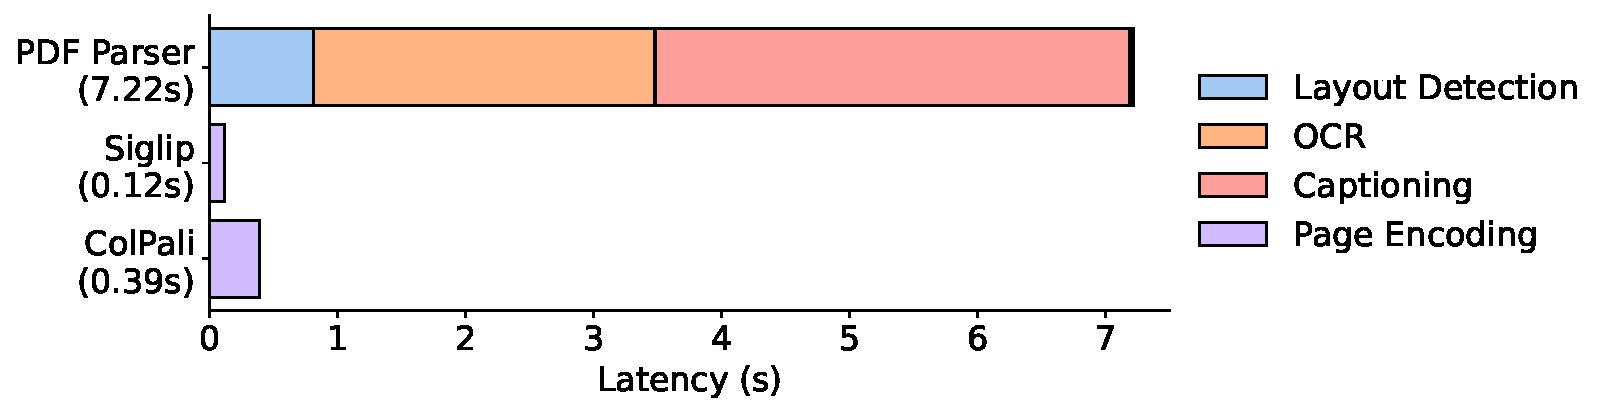
\includegraphics[width = 0.85\linewidth]{images/colpali_images/latency_comparison.pdf}
    \caption[Offline indexing latency comparison]{Offline document indexing with \textit{ColPali} is much simpler and faster compared to standard retrieval methods. The PDF Parser results are obtained following the \textit{Unstructured} settings with BGE-M3 detailed in \autoref{subsection:baseline_models}. All indexing speeds are averaged per-page latencies. More details in \autoref{paragraph:latency_app}}.
    \label{fig:latency-comparison}
\end{figure}




\section{Late interaction based Vision Retrieval}

% We propose adapting recent VLMs that have shown strong document understanding potential for multi-modal retrieval. 

% In this work, we aim to extract meaningful multi-vectorial representations of documents, relying solely on the image representation. Our proposed architecture design is presented in Figure 1.


\subsection{Architecture}
\label{subsection:colpali:architecture}


\textbf{Vision-Language Models.}
Encouraged by their strong document understanding capabilities, we propose adapting recent VLMs for retrieval. The key concept is to leverage the alignment between output embeddings of text and image tokens acquired during multi-modal fine-tuning. 
% We hypothesize that using the LLM text backbone to further encode the input image patches will integrate world-knowledge and reasoning capabilities that are key to understanding complex tables or charts. 
To this extent, we introduce \textit{ColPali}, a Paligemma-3B extension that is capable of generating ColBERT-style multi-vector representations of text and images (\autoref{fig:colpali_architecture}).
PaliGemma-3B is a strong candidate due to its small size, the many released checkpoints fine-tuned for different image resolutions and tasks, and the promising performances on various document understanding benchmarks. 
We add a projection layer to map each of the language model's output token embeddings (whether from text or image tokens)  to a vector space of reduced dimension $D = 128$ as used in the ColBERT paper \sidecite{khattab_colbert_2020} to keep lightweight bag-of-embedding representations.


\noindent\textbf{Late Interaction.}
% NOTE: archived because the R^D doesn't display properly.
% Let $q$ be the user query and $p$ a given document page. Let $\mathbf{E_q}_{(1:N_q)} = \left( \mathbf{E_q}^{(1)}, \ldots, \mathbf{E_q}^{(N_q)} \right) \in \left( \mathbb{R}^D \right)^{N_q}$ and $\mathbf{E_p}_{(1:N_p)} = \left( \mathbf{E_p}^{(1)}, \ldots, \mathbf{E_p}^{(N_p)} \right) \in \left( \mathbb{R}^D \right)^{N_p}$ their multi-vector representation in the common embedding space of dimension $D$.
Given query $q$ and document $d$, we denote as $\mathbf{E_q} \in \mathbb{R}^{{N_q} \times D}$ and $\mathbf{E_d} \in \mathbb{R}^{N_d \times D}$ their respective multi-vector representation in the common embedding space $\mathbb{R}^D$, where $N_q$ and $N_d$ are respectively the number of vectors in the query and in the document page embeddings. The late interaction operator, $\text{LI} \left( q, d \right)$, is the sum over all query vectors $\mathbf{E_{q}}^{(j)}$, of its maximum dot product $\langle \cdot | \cdot \rangle$ with each of the $N_d$ document embedding vectors $\mathbf{E_d}_{(1:N_d)}$.

\begin{equation}
    \text{LI} \left( q, d \right) = \sum_{i \in [|1, N_q|]} \max_{j \in [|1, N_d|]} \langle \mathbf{E_{q}}^{(i)} | \mathbf{E_{d}}^{(j)} \rangle
\label{eq:colbert_maxsim_score}
\end{equation}

% \ptitle{Contrastive batched loss: negative log of the softmax of the ratio of positive score to the negative scores}

\noindent\textbf{Contrastive Loss.}
The Late Interaction operation is fully differentiable, enabling backpropagation.
Let a batch $\left\{ q_k, d_k \right\}_{k \in [|1, b |]}$ composed of $b$ query-page pairs, where for all $k \in [|1, b|]$, the document page $d_k$ is the document corresponding to query $q_k$. 
% Thus, following the work of \citealt{sohn_improved_2016}, we can construct $b(b-1)$ negative pairs for this batch: the $\left\{ q_k, d_l \right\}_{k \neq l}$ (\textit{in-batch negatives}).
Following \sidecite{khattab_colbert_2020}, we define our in-batch contrastive loss $\mathcal{L}$ as the softmaxed cross-entropy of the positive scores $s_k^+ = \text{LI} \left( q_k, d_k \right)$ w.r.t. to the maximal in-batch negative scores $s_k^- = \max \limits_{l, l \neq k} \hspace{3mm} \text{LI} \left( q_k, d_l \right) $\sidenote{We reformulate the loss to leverage the numerically stable \texttt{softplus} function where $\texttt{softplus(x)} =  \log \left( 1 + \exp \left( x \right)\right)$}:

% \begin{equation}
%     \mathcal{L} = \frac{1}{b} \sum_{k=1}^{b} \texttt{softplus} \left( s_k^- - s_k^+ \right)
%     \label{equation:colpali_loss_final}
% \end{equation}



% NOTE: Full equation -> excluded because doesn't fit the column.
% \begin{equation}
%     \mathcal{L} = -\frac{1}{b} \sum_{k=1}^{b} \log \left[ \frac{\exp \left( s \left( q_k, p_k \right) \right)}{\exp \left( s \left( q_k, p_k \right) \right) + \exp \left( \max \limits_{l \in [|1, \ldots, b|] \atop l \neq k} \[ s \left( q_k, p_l \right) \] \right) } \right]
%     \label{equation:colpali_loss_full}
% \end{equation}

\begin{equation}
    \mathcal{L} = -\frac{1}{b} \sum_{k=1}^{b} \log \left[ \frac{\exp \left( s_k^+ \right)}{\exp \left( s_k^+ \right) + \exp \left( s_k^- \right)} \right] = \frac{1}{b} \sum_{k=1}^{b} \log \left( 1 + \exp \left( s_k^- - s_k^+ \right) \right)
    \label{equation:colpali_loss_full}
\end{equation}

% For all $k \in [|1, b|]$, let $s_k^+ = s(q_k, p_k)$ and $s_k^- = \max \limits_{l \in [|1, \ldots, b|] \atop l \neq k} \left( s(q_k, p_l) \right)$.



\subsection{Model training}

\noindent\textbf{Dataset.} Our training dataset of 118,695 query-page pairs is comprised of train sets of openly available academic datasets ($63\%$) and a synthetic dataset made up of pages from web-crawled PDF documents and augmented with VLM-generated (Claude-3 Sonnet) pseudo-questions ($37\%$). Dataset split details are given in \autoref{subsection:training_dataset}.
Our training set is fully English by design, enabling us to study zero-shot generalization to non-English languages\sidenote{Multilingual data is present in the pretraining corpus of the language model (Gemma-2B) and potentially occurs during PaliGemma-3B's multimodal training.}. We explicitly verify no multi-page PDF document is used both \textit{ViDoRe} and in the train set to prevent evaluation contamination. A validation set is created with $2\%$ of the samples to tune hyperparameters. We openly release the training dataset\sidenote{\url{https://huggingface.co/datasets/vidore/colpali_train_set}} for reproducibility and to encourage further research. 

\noindent\textbf{Parameters.} All models are trained for 1 epoch on the train set. Unless specified otherwise, we train models in \texttt{bfloat16} format, use low-rank adapters (LoRA, \sidecite{hu2021loralowrankadaptationlarge}) with $\alpha=32 $ and $r=32$ on the transformer layers from the language model, as well as the final randomly initialized projection layer, and use a \texttt{paged\_adamw\_8bit} optimizer. We train on an 8 GPU setup with data parallelism, a learning rate of $5e-5$ with linear decay with 2.5\% warmup steps, and a batch size of 32.

% Our reference model is ColPali with 1024 image patches, trained with memory tokens, a pairwise CE loss, a frozen vision component and an exclusively English training set.

\noindent\textbf{Query Augmentation.} As in \sidecite{khattab_colbert_2020}, we append 5 \texttt{<unused0>} tokens to the query tokens to serve as a soft, differentiable query expansion or re-weighting mechanism. 
%We do the same for the image patches, drawing inspiration from \sidecite{darcet_vision_2023}.

% We also explore the effect of adding the table and the figures to a naive baseline of only OCR. 

\section{Results}
\label{section:colpali:results}




\begin{table*}[ht]
    \centering
    
    \resizebox{\textwidth}{!}{%
    \begin{tabular}{ll@{\hskip 0.5em}l@{\hskip 0.5em}l@{\hskip 0.5em}l@{\hskip 0.5em}l@{\hskip 0.5em}l@{\hskip 0.5em}l@{\hskip 0.5em}l@{\hskip 0.5em}l@{\hskip 0.5em}l|@{\hskip 0.5em}l}

\toprule
 & \textbf{ArxivQ} & \textbf{DocQ} & \textbf{InfoQ} & \textbf{TabF} & \textbf{TATQ} & \textbf{Shift} & \textbf{AI} & \textbf{Energy} & \textbf{Gov.} & \textbf{Health.} & \textbf{Avg.} \\


 % Captioning$_{\tiny \texttt{e5-large}}$ & 30.9\textcolor{red!75!black}{\tiny $\downarrow$-4.2} & 24.0\textcolor{red!75!black}{\tiny $\downarrow$-5.8} & 62.3\textcolor{green!75!black}{\tiny $\uparrow$0.8} & 54.3\textcolor{green!75!black}{\tiny $\uparrow$29.3} & 37.6\textcolor{red!75!black}{\tiny $\downarrow$-11.3} & 44.0\textcolor{red!75!black}{\tiny $\downarrow$-3.0} & 76.0\textcolor{red!75!black}{\tiny $\downarrow$-3.0} & 71.0\textcolor{red!75!black}{\tiny $\downarrow$-5.0} & 70.0\textcolor{red!75!black}{\tiny $\downarrow$-5.0} & 72.0\textcolor{red!75!black}{\tiny $\downarrow$-9.0} \\



\midrule
    \multicolumn{0}{l}{\textbf{\texttt{Unstructured} \tiny text-only}}&&&&&&&&&&&\\
- BM25 & - & 34.1 & - & - & 44.0 & 59.6 & 90.4 & 78.3 & 78.8 & 82.6 &-\\
- BGE-M3 & - & 28.4\textcolor{red!75!black}{\tiny $\downarrow$5.7} & - & - & 36.1\textcolor{red!75!black}{\tiny $\downarrow$7.9} & 68.5\textcolor{green!75!black}{\tiny $\uparrow$8.9} & 88.4\textcolor{red!75!black}{\tiny $\downarrow$2.0} & 76.8\textcolor{red!75!black}{\tiny $\downarrow$1.5} & 77.7\textcolor{red!75!black}{\tiny $\downarrow$1.1} & 84.6\textcolor{green!75!black}{\tiny $\uparrow$2.0} & -\\
\\
\multicolumn{0}{l}{\textbf{\texttt{Unstructured} \tiny+ OCR}}&&&&&&&&&&&\\
- BM25 & 31.6 & 36.8 & 62.9 & 46.5 & 62.7 & 64.3 & 92.8 & 85.9 & 83.9 & 87.2 & 65.5\\
- BGE-M3 & 31.4\textcolor{red!75!black}{\tiny $\downarrow$0.2} & 25.7\textcolor{red!75!black}{\tiny $\downarrow$11.1} & 60.1\textcolor{red!75!black}{\tiny $\downarrow$2.8} & 70.8\textcolor{green!75!black}{\tiny $\uparrow$24.3} & 50.5\textcolor{red!75!black}{\tiny $\downarrow$12.2} & \textbf{73.2}\textcolor{green!75!black}{\tiny $\uparrow$8.9} & 90.2\textcolor{red!75!black}{\tiny $\downarrow$2.6} & 83.6\textcolor{red!75!black}{\tiny $\downarrow$2.3} & 84.9\textcolor{green!75!black}{\tiny $\uparrow$1.0} & 91.1\textcolor{green!75!black}{\tiny $\uparrow$3.9} & 66.1\textcolor{green!75!black}{\tiny $\uparrow$0.6}\\
\\
\multicolumn{0}{l}{\textbf{\texttt{Unstructured} \tiny+ Captioning}}&&&&&&&&&&&\\
- BM25 & 40.1 & 38.4 & 70.0 & 35.4 & 61.5 & 60.9 & 88.0 & 84.7 & 82.7 & 89.2 
& 65.1\\
- BGE-M3 & 35.7\textcolor{red!75!black}{\tiny $\downarrow$4.4} & 32.9\textcolor{red!75!black}{\tiny $\downarrow$5.4} & 71.9\textcolor{green!75!black}{\tiny $\uparrow$1.9} & 69.1\textcolor{green!75!black}{\tiny $\uparrow$33.7} & 43.8\textcolor{red!75!black}{\tiny $\downarrow$17.7} & 73.1\textcolor{green!75!black}{\tiny $\uparrow$12.2} & 88.8\textcolor{green!75!black}{\tiny $\uparrow$0.8} & 83.3\textcolor{red!75!black}{\tiny $\downarrow$1.4} & 80.4\textcolor{red!75!black}{\tiny $\downarrow$2.3} & 91.3\textcolor{green!75!black}{\tiny $\uparrow$2.1} & 67.0\textcolor{green!75!black}{\tiny $\uparrow$1.9}\\
    \midrule
    % \textbf{Multimodal emb.} &\\
    \multicolumn{0}{l}{\textbf{Contrastive VLMs}}&&&&&&&&&&&\\
    Jina-CLIP & 25.4 & 11.9 & 35.5 & 20.2 & 3.3 & 3.8 & 15.2 & 19.7 & 21.4 & 20.8 & 17.7 \\
    Nomic-vision & 17.1 & 10.7 & 30.1 & 16.3 & 2.7 & 1.1 & 12.9 & 10.9 & 11.4 & 15.7 & 12.9\\
    SigLIP \tiny(Vanilla)& 43.2 & 30.3 & 64.1 & 58.1 & 26.2 & 18.7 & 62.5 & 65.7 & 66.1 & 79.1 & 51.4 \\
\midrule
\multicolumn{0}{l}{\textbf{Ours}}&&&&&&&&&&&\\
SigLIP \tiny(Vanilla)& 43.2 & 30.3 & 64.1 & 58.1 & 26.2 & 18.7 & 62.5 & 65.7 & 66.1 & 79.1 & 51.4 \\
BiSigLIP \tiny (+fine-tuning) & 58.5\textcolor{green!75!black}{\tiny $\uparrow$15.3} & 32.9\textcolor{green!75!black}{\tiny $\uparrow$2.6} & 70.5\textcolor{green!75!black}{\tiny $\uparrow$6.4} & 62.7\textcolor{green!75!black}{\tiny $\uparrow$4.6} & 30.5\textcolor{green!75!black}{\tiny $\uparrow$4.3} & 26.5\textcolor{green!75!black}{\tiny $\uparrow$7.8} & 74.3\textcolor{green!75!black}{\tiny $\uparrow$11.8} & 73.7\textcolor{green!75!black}{\tiny $\uparrow$8.0} & 74.2\textcolor{green!75!black}{\tiny $\uparrow$8.1} & 82.3\textcolor{green!75!black}{\tiny $\uparrow$3.2} & 58.6\textcolor{green!75!black}{\tiny $\uparrow$7.2}\\

BiPali \tiny (+LLM) & 56.5\textcolor{red!75!black}{\tiny $\downarrow$-2.0} & 30.0\textcolor{red!75!black}{\tiny $\downarrow$-2.9} & 67.4\textcolor{red!75!black}{\tiny $\downarrow$-3.1} & 76.9\textcolor{green!75!black}{\tiny $\uparrow$14.2} & 33.4\textcolor{green!75!black}{\tiny $\uparrow$2.9} & 43.7\textcolor{green!75!black}{\tiny $\uparrow$17.2} & 71.2\textcolor{red!75!black}{\tiny $\downarrow$-3.1} & 61.9\textcolor{red!75!black}{\tiny $\downarrow$-11.7} & 73.8\textcolor{red!75!black}{\tiny $\downarrow$-0.4} & 73.6\textcolor{red!75!black}{\tiny $\downarrow$-8.8} & 58.8\textcolor{green!75!black}{\tiny $\uparrow$0.2}\\
\textit{ColPali} \tiny (+Late Inter.) & \textbf{79.1}\textcolor{green!75!black}{\tiny $\uparrow$22.6} & \textbf{54.4}\textcolor{green!75!black}{\tiny $\uparrow$24.5} & \textbf{81.8}\textcolor{green!75!black}{\tiny $\uparrow$14.4} & \textbf{83.9}\textcolor{green!75!black}{\tiny $\uparrow$7.0} & \textbf{65.8}\textcolor{green!75!black}{\tiny $\uparrow$32.4} & \textbf{73.2}\textcolor{green!75!black}{\tiny $\uparrow$29.5} & \textbf{96.2}\textcolor{green!75!black}{\tiny $\uparrow$25.0} & \textbf{91.0}\textcolor{green!75!black}{\tiny $\uparrow$29.1} & \textbf{92.7}\textcolor{green!75!black}{\tiny $\uparrow$18.9} & \textbf{94.4}\textcolor{green!75!black}{\tiny $\uparrow$20.8} & \textbf{81.3}\textcolor{green!75!black}{\tiny $\uparrow$22.5}\\

\bottomrule

\end{tabular}}


    \caption[Baseline and \textit{ViDoRe} evaluation]{\textbf{Comprehensive evaluation of baseline models and our proposed method on \textit{ViDoRe}.} Results are presented using nDCG@5 metrics, and illustrate the impact of different components. Text-only metrics are not computed for benchmarks with only visual elements.} 
    \label{table:colpali:results}
\end{table*}



\subsection{Performance (R1)}
\label{subsection:performace}

% We iteratively construct \textit{ColPali}, starting from an off-the-shelf SigLIP model (\autoref{table:results}).

We show performance is achieved iteratively through the combination of three factors; (1) a carefully crafted task-specific dataset, (2) pairing a pretrained LLM to a vision model to better leverage text semantics from the image, and (3) using multi-vector embeddings rather than a single vector representation to better capture the vast amount of visual information present in a document.
 
%\noindent\textbf{BiSigLIP: Improving a strong model.} SigLIP\sidenote{\url{https://huggingface.co/google/siglip-so400m-patch14-384}} is a strong vision-language bi-encoder model, pretrained on the English split of WebLI \sidecite{chen_pali-3_2023}, a corpus of billions of image-text pairs. We find that SigLIP largely outperforms both Jina CLIP and Nomic-vision on document retrieval tasks. Further fine-tuning the textual component of this model on our document-oriented dataset (BiSigLIP) yields clear improvements across the board, particularly on figure retrieval (ArxivQA) and table retrieval tasks (TabFQuAD).
\noindent\textbf{Fine-tuning a Vision Model on a document retrieval oriented dataset: \textit{BiSigLIP}.} SigLIP\sidenote{\url{https://huggingface.co/google/siglip-so400m-patch14-384}} is a strong vision-language bi-encoder producing single vector embeddings, and pretrained on billions of image-text pairs from the English split of WebLI \sidecite{chen_pali-3_2023}. Further fine-tuning the textual component of this model on our document-oriented dataset (BiSigLIP) yields clear improvements across the board, particularly on figure retrieval (ArxivQA) and table retrieval tasks (TabFQuAD).

% \noindent\textbf{BiPali: Pairing with a language model.} In the PaliGemma model architecture, SigLIP-generated patch embeddings are fed to a text language model to obtain LLM contextualized output patch embeddings.\sidenote{Note that the SigLIP model used in PaliGemma slightly differs in terms of number patches -  1024 patches for PaliGemma's vision encoder, and 729 for the standalone SigLIP model.} We average pool these representations to obtain a single dense vector, effectively creating a PaliGemma bi-encoder model (BiPali). After fine-tuning on the training dataset, we obtain a model that performs slightly worse in English than the tuned BiSigLIP variant. This can be explained by the fact that contrary to SigLIP, the original PaliGemma is not trained on contrastive matching tasks, but rather on next token prediction. Our contrastive fine-tuning phase on 119K images to transform PaliGemma into a bi-encoder is 5 orders of magnitude smaller than SigLIP's original contrastive training. However, we see notable improvements in French tasks, indicating that BiPali's LLM (Gemma 2B) helps multilingual text understanding. This is particularly notable as our training dataset does not contain non-English samples.

\noindent\textbf{Feeding image patches to a LLM: \textit{BiPali}.} In the PaliGemma model architecture, SigLIP-generated patch embeddings are fed to a text language model and we can obtain LLM contextualized output patch embeddings.\sidenote{Note that the SigLIP model used in PaliGemma slightly differs in terms of number patches -  1024 patches for PaliGemma's vision encoder, and 729 for the standalone SigLIP model.} This technique aligns the image token representations with the text token embeddings in the LLM's embeddings space, and augments the vision model embeddings with the language model's text understanding capabilities. We average pool these representations to obtain a single dense vector, effectively creating a PaliGemma bi-encoder model (BiPali). After fine-tuning on the training dataset, we obtain a model that performs slightly worse in English than the tuned BiSigLIP variant.\sidenote{This can be explained by the fact that contrary to SigLIP, the original PaliGemma is not trained on contrastive matching tasks, but rather on next token prediction. Our contrastive fine-tuning phase on 119K images to transform PaliGemma into a bi-encoder is 5 orders of magnitude smaller than SigLIP's original contrastive training.} However, we see notable improvements in French tasks, indicating that BiPali's LLM (Gemma 2B) helps multilingual text understanding. This is particularly notable as our training dataset does not contain non-English samples.

% \noindent\textbf{\textit{ColPali}: Adding Late Interaction.}
% One benefit of inputting image patch embeddings through a language model is that they are natively mapped to a latent space similar to textual input (query). This enables leveraging the ColBERT strategy to compute interactions between text tokens and image patches, which enables a step-change improvement in performance compared to BiPali. 
% Results in \autoref{table:results} show that our \textit{ColPali} model also largely outperforms the strong baselines based on \texttt{Unstructured} and captioning, as well as all evaluated text-image embedding models. The difference is particularly stark on the more visually complex benchmark tasks, such as InfographicVQA, ArxivQA, and TabFQuAD representing respectively infographics, figures, and tables. However, text-centric documents are also better retrieved by the \textit{ColPali} models across all evaluated domains and languages, making our approach the overall best-performing document-retrieval model.

\noindent\textbf{Leveraging Multi-Vector Embeddings through Late Interaction: \textit{ColPali}.}
One benefit of inputting image patch embeddings through a language model is that they are natively mapped to a latent space similar to the textual input (query). This enables leveraging the ColBERT strategy to construct one embedding per image patch token, and at inference compute all interactions between text tokens and image patches, resulting in a step-change improvement in performance compared to BiPali. 
Results in \autoref{table:colpali:results} show that our \textit{ColPali} model also largely outperforms the strong baselines based on \texttt{Unstructured} and captioning, as well as all evaluated text-image embedding models. The difference is particularly stark on the more visually complex benchmark tasks, such as InfographicVQA, ArxivQA, and TabFQuAD, respectively representing infographics, figures, and tables. However, text-centric documents are also better retrieved by the \textit{ColPali} models across all evaluated domains and languages, making our approach the overall best-performing document-retrieval model.

\noindent\textbf{Negative Results.} For extensiveness, we also train ColSigLIP, a late interaction variant of the BiSigLIP model but obtain abysmal performances. We attribute this to the large gaps w.r.t. SigLIP's pre-training, in which only a pooled latent representation is used in the contrastive loss, which does not optimize the representations of individual patch and token embeddings. Similarly, we train a BiSigLIP$_{PaliGemma}$ variant, in which we retrieve the image representations from the SigLIP model that has been further updated by PaliGemma fine-tuning, and use the text representations from PaliGemma's text model. After fine-tuning on our dataset, performance is severely inferior to SigLIP$_{Vanilla}$ which simply encodes with SigLIP's original text and vision components. This indicates a logical misalignment between SigLIP embeddings, and Gemma embeddings after PaliGemma training. We detail these results in \autoref{subection:additional_results}.

%Add training infomation out-of-domain
% \noindent\textbf{Language Modeling helps.} Compared to a standard contrastive vision-language model like SigLIP, further fine-tuned on the same dataset, we are interested in observing the performance improvement obtained by feeding SigLIP tokens into a text language model. We denote the standard SigLIP bi-encoder as BiSigLIP and the bi-encoder version of ColPali as BiPali. In both models, we average pool the representations of respectively the query tokens and the image tokens.\sidenote{We have tried variants such as keeping only the last token but mean pooling yields the best results.} We also baseline BiSigLIP, the BiSigLIP encoder that has been further pre-trained as part of the PaliGemma model to analyze whether continued training with a generative language modeling objective helps refine image embeddings. Our results show the clear improvements of BiPali over BiSigLIP, demonstrating that the language model brings refined semantic understanding capabilities.
% \noindent\textbf{Late Interaction helps.} Also interesting are the performance gains obtained through the late interaction retrieval scheme. We show that compared to the bi-encoder BiPali, ColPali shows vastly improved metric performance across the board. 
% \noindent\textbf{Zero-shot multilingualism.}
% Images are particularly good candidates for such a scheme thanks to their fixed size


\subsection{Latencies \& Memory Footprint}
\label{subsection:latency}
% Hugues

% TODO: https://arxiv.org/abs/2304.01982

\noindent \textbf{Online Querying. (R2)} Logically, querying latencies differ between \textit{ColPali} and a BGE-M3 embedding model. For BGE, encoding takes about $22$ ms for 15 tokens, while encoding a query with \textit{ColPali}'s language model takes about $30$ ms\sidenote{Computed for a batch size of $1$ (online), and averaged over 1000 queries. See \autoref{paragraph:latency_app}}. For smaller corpus sizes, computing the late interaction operation induces marginally small overheads ($\approx 1$ ms per 1000 pages in the corpus), and the cosine similarity computation between bi-encoder vectors is even faster. Optimized late interaction engines \sidecite{santhanam_plaid_2022, lee_rethinking_2023} enable to easily scale corpus sizes to millions of documents with reduced latency degradations.


\noindent\textbf{Offline Indexing. (R3)} 
Standard retrieval methods using bi-encoders represent each chunk as a single vector embedding, which is easy to store and fast to compute. However, processing a PDF to get the different chunks is the most time-consuming part (layout detection, OCR, chunking), and using captioning to handle multimodal data will only exacerbate this already lengthy process. On the other hand, \textit{ColPali} directly encodes pages from their image representation. Although the model is larger than standard retrieval encoders, skipping the preprocessing allows large speedups at indexing\sidenote{Measures a NVIDIA L4 GPU, averaged on 100 pages, with a batch size of 4 pages for \textit{ColPali} and 8 text chunks for Bi-Encoders. On average, a page is divided into 2.1 chunks. See \autoref{paragraph:latency_app}.} (\autoref{fig:latency-comparison}). As pages are embedded end-to-end in single forward pass, the VRAM usage depends exclusively on the sequence length (number of patches per image) which is fixed as well, enabling efficient batching strategies to fully leverage hardware acceleration. ColPali also benefits from most LLM efficiency improvements introduced in the ecosystem such as Flash Attention \sidecite{dao2023flashattention2fasterattentionbetter}.

\noindent\textbf{Storage Footprint.} Our method requires storing a vector per image patch, along with 6 extra text tokens ``Describe the image" concatenated to image patches. We project each PaliGemma vector to a lower dimensional space ($D=128$) to maximize efficiency, leading to a memory footprint of $257.5$ KB per page (\autoref{subsection:embedding_size}). Importantly, the memory footprint of the naive ColBERT indexing strategy can be drastically improved through compression and clustering mechanisms \sidecite{santhanam_plaid_2022, clavie_reducing_2024}.

\noindent\textbf{Token pooling.}
% Multi-vector embeddings scale linearly in size with respect to the number of tokens, inducing longer indexing and search time. 
Token pooling \sidecite{clavie_reducing_2024} is a CRUDE-compliant method (document addition/deletion-friendly) that aims amountto reduce the amount of multi-vector embeddings. For ColPali, many image patches share redundant information, e.g. white background patches. By pooling these patches together, we can reduce the amount of embeddings while retaining most information. Retrieval performance with hierarchical mean token pooling on image embeddings is shown in \autoref{fig:combined_figures} (left).
With a pool factor of 3, the total number of vectors is reduced by $66.7\%$ while $97.8\%$ of the original performance is maintained. We note that the Shift dataset—composed of the most text-dense documents—is a clear outlier, showcasing more information dense documents contain less redundant patches and may be prone to worse performance degradation with such pooling techniques.

\subsection{Interpretability}
\label{subsection:similarity_maps}

% \begin{figure}
% \centering
% % \includegraphics[width=0.5\linewidth]{images/colpali_images/similarity_maps/similarity_map_energy.png} 
% 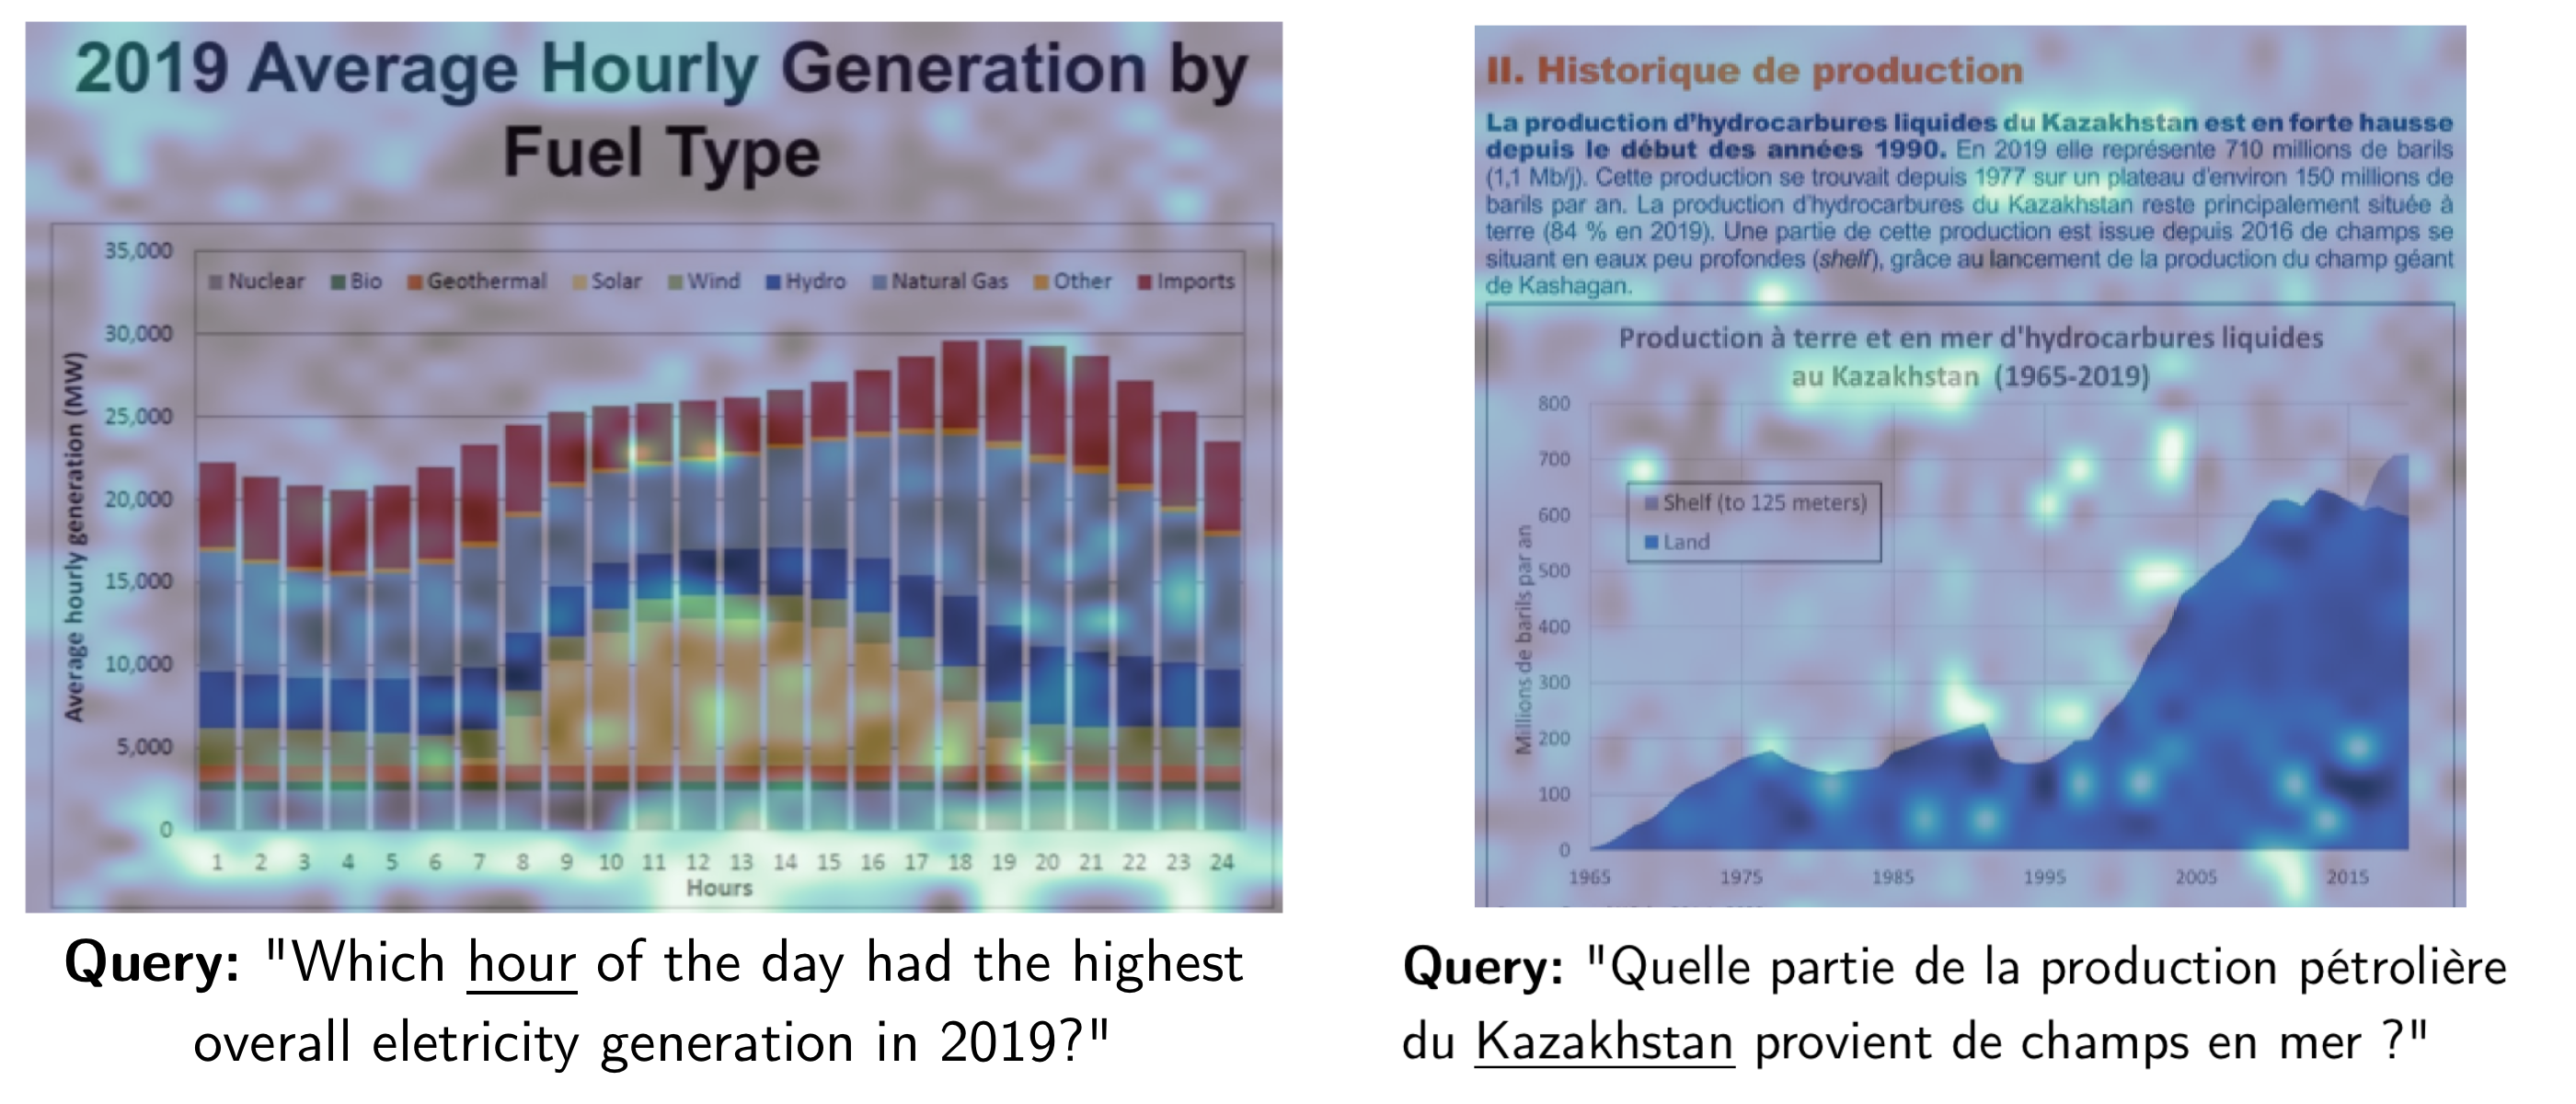
\includegraphics[width = 1\linewidth]{images/colpali_images/similarity_maps/similarity_maps.png} 
%     \caption{For each term in a user query, \textit{ColPali} identifies the most relevant document image patches (highlighted zones) and computes a query-to-page matching score. We can then swiftly retrieve the most relevant documents from a large pre-indexed corpus.}
% \label{fig:similarity_maps}
% \end{figure}


\begin{figure}
\centering
\begin{minipage}{.5\textwidth}
  \centering
  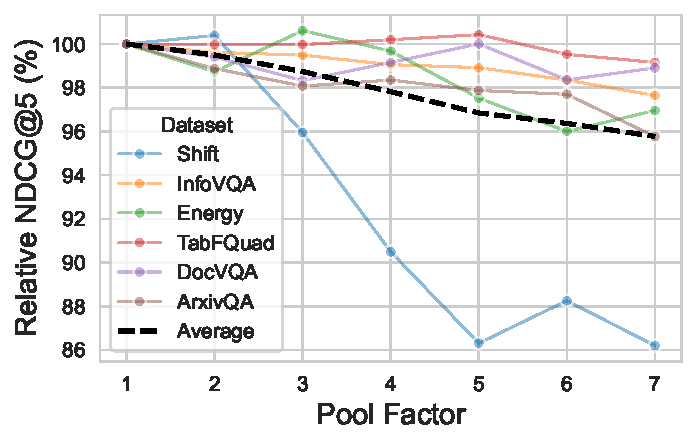
\includegraphics[width=1\linewidth]{images/colpali_images/token_pooling_ndcg.pdf}
\end{minipage}%
\begin{minipage}{.45\textwidth}
  \centering
  \includegraphics[width=0.9\linewidth]{images/colpali_images/similarity_map_energy.png}
\end{minipage}
\caption[Token pooling and interpretability]{(Left: \textbf{Token Pooling}) Relative performance degradation when reducing the number of stored embeddings per document. (Right: \textbf{Interpretability}) For each term in a user query, \textit{ColPali} identifies the most relevant document image patches (highlighted zones) and computes a query-to-page matching score.}
\label{fig:combined_figures}
\end{figure}

% \begin{figure}
% \centering
% \begin{minipage}{.45\textwidth}
%   \centering
%   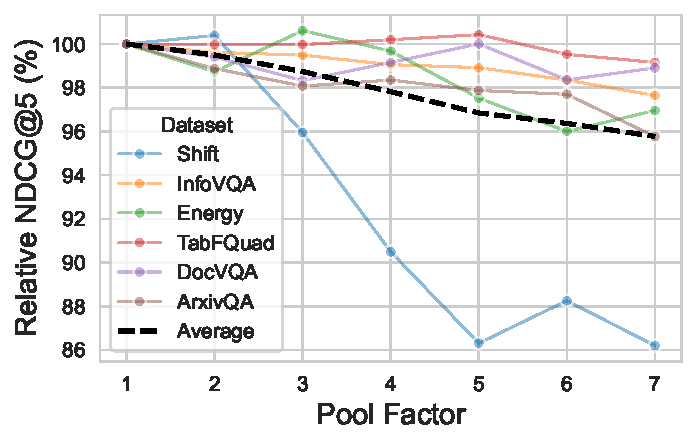
\includegraphics[width=1\linewidth]{images/colpali_images/token_pooling_ndcg.pdf}
%   \captionof{figure}{Relative performance degradation for token pooling on image embeddings generated by \textit{ColPali}.}
%   \label{fig:token-pooling}
% \end{minipage}
% \begin{minipage}{.45\textwidth}
%   \centering
%   \includegraphics[width=0.9\linewidth]{images/colpali_images/similarity_map_energy.png}
%   \captionof{figure}{For each term in a user query, \textit{ColPali} identifies the most relevant document image patches (highlighted zones) and computes a query-to-page matching score.}
%   \label{fig:similarity_maps}
% \end{minipage}%
% \end{figure}

% When we feed an image to ColPali, each image patch is mapped to a vector. Thus, the output is a sequence of $n_{\text{patch}}$ vectors. Because of the ViT positional embeddings and of the generative nature of the pre-trained LLM backbone in ColPali, we believe still have the notion of the image patch structure. Thus, we have mapped the output ColPali representation of the image to a $[0, 1]^{n_{\text{patch}}^2}$ matrix to visualize the per-patch similarity scores with a give query token. This is epitomized in \autoref{fig:similarity_map_hourly}.

%ColPali outputs a 128-dimensional vector for every input image patch (1024), which is used for late interaction matching.\


By superimposing the late interaction heatmap on top of the original image, we can visualize the most salient image patches with respect to each term of the query, yielding interpretable insights into model focus zones. As epitomized in \autoref{fig:combined_figures} (right), we observe \textit{ColPali} exhibits strong OCR capabilities as both the words \textit{``hourly"} and \textit{``hours"} present a high similarity score with the query token \texttt{<\_hour>}. We also note particular focus on other non-trivial image features such as the x-axis representing hours being salient. Other visualization examples are shown in \autoref{section:more_similarity_maps}.

% By superimposing the late interaction heatmap on top of the original image, we can visualize the most salient image patches with respect to each term of the query, yielding interpretable insights into model focus zones. In the first figure in \autoref{fig:similarity_maps}, we observe \textit{ColPali} exhibits strong OCR capabilities as both the words \textit{"hourly"} and \textit{"hours"} present a high similarity score with the query token \texttt{<\_hour>}. We also note particular focus on other non-trivial image features such as the x-axis representing hours being salient.

% Other visualization examples with similar trends of the model transcending pure OCR are shown in \autoref{section:more_similarity_maps}.

% Both similarity maps present a few white patches with high similarity scores. This behavior might first seem surprising as the white patches should not carry a meaningful signal from the original images. We believe the vectors associated with these patches share a similar role with the ViT registers \sidecite{darcet_vision_2023}, i.e.\ these patches were repurposed for internal computations and stored the global information from the whole image.


\section{Ablation study}
\label{section:ablation_study}

We run various ablations to better understand the mechanisms at play. By default, result deltas reported below refer to nDCG@5 values averaged over all ViDoRe tasks.  Detailed results in \ref{subection:model_variants}.

%\subsection{Is it better to increase model size or the number of patches ?}

%\noindent\textbf{Number of patches.} 
\noindent\textbf{Tradeoffs between model size and the number of image patches.} We train a variant of PaliGemma with half the number of image patches (512). % The number of tokens is directly linked to the resolution of the embedded image patches.
While we observe a clear performance degradation with respects to to the 1024-patch \textit{ColPali} model ($-24.8$ nDCG@5), memory usage is much lower.
%\sidenote{Yet another PaliGemma variant exists with 2048 patches, but the large memory requirements make this model impractical to train contrastitively and to run inference with.}
%\noindent\textbf{Language Model size.} 
As an alternative to PaliGemma, we train Idefics2-8B \sidecite{laurencon_what_2024}, a VLM with a similar architecture and based on a Mistral-7B \sidecite{jiang_mistral_2023} language backbone and a SigLIP vision encoder paired with a perceiver resampler. The most notable differences with PaliGemma lie in the size of the language model (2B and 7B resp.) and the number of image patches (between 512 and 2048 for PaliGemma, and 64 post-resampling for Idefics2\sidenote{With the option of adding 4 sub-image crops of 64 tokens each to the sequence, for a total of 320 tokens}). Our results suggest better language models enable more efficient representations of image embeddings - ColIdefics2 with 64 patches largely outperforms out \textit{ColPali} with 512 patches (+20.1 nDCG@5). However ColIdefics2 (64) remains less accurate than ColPali (1024) ($-4.7$ nDCG@5) while being about twice as slow in terms of training and inference latency.
%
%\noindent\textbf{Tradeoffs.} 
% Scaling the number of patches of the smaller \textit{ColPali} model from 512 to 1024, enables largely surpassing the 60-patch ColIdefics2 while being about twice as fast in terms of training and inference latency. 
These results suggest there are \textit{tradeoffs} between performance (R1), latencies during online querying (R2) and offline indexation phases (R3), and index memory size.

% \vspace{0.5cm}
\noindent\textbf{Unfreezing the vision component.} We train a \textit{ColPali} variant by also backpropagating through and updating the vision encoder and the projection layer. This leads to a slight performance degradation ($-0.7$ nDCG@5). These conclusions may change with larger scales of training data.

% \subsection{Do "query augmentation" tokens help ?}
% \vspace{0.2cm}
\noindent\textbf{Impact of ``query augmentation" tokens.} In ColBERT, special tokens are concatenated to the input query to serve as soft query augmentation buffers. Training without these tokens, we observe no significant performance difference in the English benchmarks. However, performance on the French tasks seems to improve ($+9.8$ nDCG@G on Shift, $+6.3$ nDCG@5 on TabFQuAD, \autoref{table:negative_results}).
% \sidecite{mckinzie_mm1_2024,bordes_introduction_2024,li_llava-next_2024}


% \subsection{Pairwise Cross-Entropy (CE) Loss}
% \vspace{0.2cm}
\noindent\textbf{Impact of the Pairwise CE loss.} Training with an in-batch negative contrastive loss, instead of the pairwise CE loss that only considers the hardest negative sample, leads to a slight performance degradation ($-1.6$ nDCG@5) on the aggregated benchmark.

% \vspace{0.2cm}
\noindent\textbf{Adapting models to new tasks.} Contrary to more complex multi-step retrieval pipelines, \textit{ColPali} can be trained end-to-end, directly optimizing the downstream retrieval task which greatly facilitates fine-tuning to boost performance on specialized domains, multilingual retrieval, or specific visual elements the model struggles with. To demonstrate, we add 1552 samples representing French tables and associated queries to the training set. This represents the only French data in the training set, with all other examples being kept unchanged. We see clear nDCG@5 improvements ($+2.6$) and even starker Recall@1 gains ($+5$) on the TabFQuAD benchmark, with no performance degradation on the rest of the benchmark tasks ($+0.4$ nDCG@5 overall).

\noindent\textbf{Better VLMs lead to better visual retrievers.} As improved VLMs are released, it is interesting to observe if improved performances on generative tasks translate once these models are adapted for image retrieval tasks through ColPali training strategies. We train the recently released Qwen2-VL 2B \sidecite{wang2024qwen2vlenhancingvisionlanguagemodels}, a SOTA 2 billion parameter generative VLM, with the same data and training strategy, obtaining ColQwen2-VL. To approximately match ColPali's memory requirements, we limit the number of image patches to 768, slightly less than ColPali's 1024 patches. We observe clear performance improvements of $+5.3$ nDCG@5 values over ColPali showcasing clear performance correlations between generative benchmarks performance and retrieving metrics.

\noindent\textbf{Out-of-domain generalization.} Some of the datasets in the ViDoRe benchmark have train sets, which we have integrated within the ColPali train set (eg. academic tasks). This is standard in embedding models \sidecite{wang2024improvingtextembeddingslarge, lee2024nvembedimprovedtechniquestraining}, and while ColPali also exhibits strong performance on tasks in which this is not the case (French data is never seen by the model during training for instance), it remains interesting to evaluate model performance when training is done on a fully disjoint data distribution. We train a ColPali variant solely using the recent DocMatix dataset \sidecite{laurençon2024building}, a large scale, synthetically annotated visual document question answering dataset, which we subsample to obtain a comparably-sized train set. Results on ViDoRe show the performance drop is minor ($-2.2$ nDCG@5), still outperforming the closest baseline method by over 12 points. These results showcase
ColPali generalizes well outside of its training distribution, and demonstrate that our results are not unreasonably boosted with respect to baselines (BGE-M3) that cannot be fine-tuned on the same data\sidenote{To train with data resembling the one BGE-M3 models would see at inference time would require running complex extraction pipelines for the more than 100K documents in the training set, notably relying on external proprietary captioning models which is both too costly and lengthy. This is not needed to train vision-based models.} 
%In practice, these models are most often used off-the-shelf without further fine-tuning in the majority of use cases.}

\section{Conclusions}
\label{section:colpali:conclusions_and_future_work}

In this work, we introduced the Visual Document Retrieval Benchmark (\textit{ViDoRe}), which evaluates document retrieval systems in realistic settings involving visually complex documents. We demonstrated that current retrieval pipelines and contrastive vision-language models struggle to efficiently exploit visual information embedded in documents, leading to suboptimal performance. To address this, we presented \textit{ColPali}, a novel retrieval method that leverages Vision-Language Models to create high-quality, multi-vector embeddings purely from visual document features. \textit{ColPali} largely outperforms the best existing document retrieval methods while enabling faster corpus indexing times and maintaining low querying latencies, thus circumventing many pain points of modern document retrieval applications. We hope to drive industrial adoption, and to encourage future work by publicly releasing the \textit{ViDoRe} benchmark, the data, the codebase, and all models and baselines from our work.

% hese results demonstrate the potential and the many benefits of this novel Retrieval in Vision Space concept, which could significantly alter the way document retrieval is approached in the industry moving forward. 

% Future work
% Image patch embeddings 
\noindent\textbf{Future Work.} 
% Further performance gains could be obtained by exploring sub-image decomposition \sidecite{liu_improved_2023}, optimal image patch resampling strategies \sidecite{laurencon_what_2024}, or hard-negative mining. 
%as well as training with larger batch size, 
% Next, we want to reduce the time and space footprint of our method using PLAID \sidecite{santhanam_plaid_2022} and XTR \sidecite{lee_rethinking_2023}. 
Beyond performance improvements that could be obtained through better data, backbone models or training strategies, our vision at term is to combine visual retrieval systems and visually grounded query answering to create end-to-end RAG systems that purely function from image features. This idea is supported by concurrent work \sidecite{ma2024mmlongbenchdocbenchmarkinglongcontextdocument} showcasing the strong promises of VLMs for visual QA, and may eventually become a new industrial standard for document processing. In this line of work, reliability is key, and confidence estimation techniques for Information Retrieval methods could become central to implement abstention mechanisms \sidecite{gisserotboukhlef2024trustworthyrerankingsimpleeffective}, and are particularly interesting given the information rich multi-vector scoring mechanisms of late interaction systems.
Expanding benchmarking efforts to cover more languages, modalities, and tasks is also a crucial future research direction \sidecite{jiang2024vlm2vectrainingvisionlanguagemodels}.
 
% , without having to reuse the original image.

% Similarly, as in GritLM, we could also envision a model that is performant both for retrieval and generative modeling.


% Mention it'd be great to test the two-stage e2e top-k retrieval from COlBERT's paper section 3.6

% Experiment aspect-preserving ViT grid = experiment any resolution
% \sidecite{dehghani_patch_2023}


% % Experiment sub-image decomposition
% Sub-image decomposition \sidecite{liu_improved_2023}
% Super sub-image decomposition \sidecite{li_llava-next_2024}

% % Add registers in the ViT
% Registers in the ViT \sidecite{darcet_vision_2023}


% % Experiment w/ LLM-as-encoders
% Try the better LLM fine-tuning with masking etc..
% \sidecite{behnamghader_llm2vec_2024}


% % Analyze the impact of resolution
% \sidecite{dou_empirical_2021}
% \sidecite{mckinzie_mm1_2024}

% Hard negative mining

% Recycle the model for different use cases (multi-adapters)
% GritLM
% webpages


% \section*{Limitations}
% \label{section:limitations}

% \noindent\textbf{Focus.} In this work, we evaluate models on document retrieval tasks, covering several modalities (figures, text, tables, infographics). We however primarily focus on PDF-type documents, and evaluating systems on image retrieval with documents stemming from web page screenshots or hand-written documents might be an interesting generalization. We also focus on high-resource languages (English and French) and although we have shown the capacity of the \textit{ColPali} model to generalize to languages outside of its fine-tuning set, it is unclear how the model would perform on languages that are not as represented in the model's language backbone. Finally, our setup assumes relevant documents exist, but abstention methods for Information Retrieval systems might be interesting to explore in more practical settings in which confidence estimation might be important \sidecite{gisserotboukhlef2024trustworthyrerankingsimpleeffective}.

% % memory requirementd --> deployment difficulty
% \noindent\textbf{Support.} This work relies on multi-vector retrieving derived from the ColBERT late interaction mechanism. Although some vector databases support late interaction engines\sidenote{\href{https://vespa.ai/}{Vespa Engine}, \href{https://github.com/bclavie/RAGatouille}{RAGatouille}, \href{https://github.com/qdrant/qdrant}{QDrant}, \href{https://github.com/stanford-futuredata/colbert}{colbert.ai}}, many widely used vector retrieval frameworks do not propose native multi-vector support, and some engineering infrastructure efforts may be required to adapt them to work with \textit{ColPali} (or ColBERT) models. 

% \noindent\textbf{Data.} In the creation of \textit{ViDoRe}, we partially rely on synthetic query generation based on a commercial large language model, which may induce some amount of bias in the generated queries. To compensate for this, we have iterated on the prompting strategy and given real query examples to the models to help ground generation in realistic settings. We have further manually verified all synthetic queries through a lengthy process to validate their relevance and their quality. Our benchmark also includes many benchmark tasks with no synthetic data, and result trends observed between all tasks are correlated, further confirming the coherence of our benchmark design.



% \section*{Ethics Statement}

% \noindent\textbf{Carbon Footprint.} Our work fully leverages prior pretrained models and training is not particularly compute-intensive. Furthermore, we rely on low-rank adapters to further reduce the computational resources needed, both during training and for storage. Overall, a training run represents about 40 hours of Mi250x AMD GPUs. Our experiments, in total, represent 1405 Mi250x GPU hours from highly efficient compute clusters running on low-carbon nuclear energy, representing a total of around 15kg CO2 eq.

% \noindent\textbf{Impact.} We believe our work could have a strong impact on improving industrial document retrieval systems. Our method is efficient, performs well, and the additional support towards visually rich information from documents could go a long way in unlocking knowledge sources previously difficult to index or query.

\section*{Reproducibility Statement}

For transparency, reproducibility and to foster future work, we release our training data, model checkpoints (adapters), entire codebase, and complete evaluation benchmark under MIT licenses as detailed in the main paper. We also host a public \textit{ViDoRe} leaderboard\sidenote{\url{https://huggingface.co/spaces/vidore/vidore-leaderboard}} to foster concurrent work in the space. The supplementary material further details training configurations for our models (also specified in HuggingFace model repositories), and dives into the process we used to generate synthetic data, how latency computations are performed, as well as provides further detailed evaluation results.



\section*{Acknowledgements}

This work is partially supported by Illuin Technology, and by a grant from ANRT France. This work was performed using HPC resources from the CINES ADASTRA through Grant 2024-AD011015443 and from IDRIS with grant 2024-AD011015724R1.
We extend our warm thanks to Jonathan Dong, Caio Corro, Victor Pellegrain and Ender Konukoglu for their valuable feedback on the paper.
